\chapter{Delta potential} \label{chapter-dirac}
In this chapter we will examine the Landau Hamiltonian with a potential perturbation (see definition \ref{defn-perturb-potential}), formally given by the potential $V(x) = \alpha\,\delta_{x_0}$, i.e. the Dirac delta in $x=x_0$, scaled by $\alpha \in \R$. Since such a potential is a distribution and not a locally integrable function, the Hamiltonian is rigorously defined as:
\begin{equation*}
    \big( H_\alpha \psi \big)(x, y) = \left( -\pd{^2}{x^2} + \big( \i\pd{}{y} + bx \big)^2 \right) \; \psi(x,y)
    \quad \text{a.e.\footnotemark on } (\R \setminus \{ x_0 \}) \times \R
\end{equation*}
\footnotetext{The pointwise equality is to be understood \textit{almost everywhere} with respect to the Lebesgue measure on $\R^2$.}
with a domain given by the conditions
\begin{gather*}
    \psi \in W^{1,2}(\R^2) \; \cap \; W^{2,2}\big( \,(\R \setminus \{ x_0 \}) \times \R \, \big) \: ,
    \\[5pt]
    \lim_{x \to x_0 +} \!\psi'(x,y)\; - \lim_{x \to x_0 -} \!\psi'(x,y) = \alpha \lim_{x \to x_0} \!\psi(x, y)
    \quad \text{for a.e. } y \: ,\footnotemark
    \\[5pt]
    \int_{\R^2} x^2 \, \big|\, \psi(x,y) \,\big|^2 \, \d{x}\d{y} < \infty \: .
\end{gather*}
\footnotetext{The equality holds for \textit{almost every} $y$ and $\lim_{x\to x_0}$ means the \textit{essential} limit with respect to the Lebesgue measure on $\R$.}
Then, by an approach analogous to \eqref{eqn-vague-direct-integral-decomp}, one can show that $H_\alpha$ is unitarily equivalent to a direct integral:
\begin{equation*}
    H_\alpha \simeq \int^\oplus_\R \Hf_\alpha(p) \d{p} \: ,
\end{equation*}
where $\Hf_\alpha(p)$ is a fibre Hamiltonian satisfying very similar conditions to those of~$H_\alpha$, that is, for almost every $p \in \R$:
\begin{gather*}
    \big( \Hf_\alpha(p) \, \varphi \big)(x)
    = -\varphi''(x)
    + \big( b \, x + p \big)^2 \, \varphi(x) \: ,
    \numberthis\label{eqn-dirac-fibre-hamiltonian}
    \\[15pt]
    \varphi \in W^{1,2}(\R) \; \cap \; W^{2,2}( \R \setminus \{ x_0 \}) \: ,
    \\[5pt]
    \lim_{x \to x_0+} \varphi'(x) - \lim_{x \to x_0-} \varphi'(x) = \alpha \, \lim_{x \to x_0} \varphi(x),
    \\[3pt]
    \int_\R x^2 \, |\varphi(x)|^2 \d{x} < \infty \: .
\end{gather*}
Before we start investigating the spectrum, we need to show that the problem is well-posed, i.e. that the Hamiltonian $H_\alpha$ is self-adjoint and bounded from below. Then we will show that the spectrum of $\Hf_\alpha(p)$ is discrete for every $p$, and only after that we will investigate the continuity of the spectrum of $H_\alpha$.

\section{Well-posedness} \label{section-dirac-well-posedness}
It is straightforward to check that the fibre Hamiltonian is bounded from below:
\begin{align*}
    (\varphi, \, \Hf_\alpha(p) \, \varphi)
    &= \int_\R \overline{\varphi}(x) \, \Big( -\varphi''(x) + (b x + p)^2 \varphi(x) \Big) \d{x}
    \\
    &= -\int_\R \overline{\varphi} \varphi''
    + \int_\R (b x + p)^2 \;\, \big|\varphi(x)\big|^2 \; \d{x}
    \\
    &\geq -\int_\R \overline{\varphi} \varphi''
    = \int_\R \overline{\varphi}' \varphi'
    - [\overline{\varphi}\varphi']_{-\infty}^{x_0}
    - [\overline{\varphi}\varphi']_{x_0}^{\infty}
    \\
    &= \norm{\varphi'}_{L^2(\R)}^2
    + \overline{\varphi}(x_0)
    \, \big( \varphi'(x_0+) - \varphi'(x_0-) \big)
    \\
    &= \norm{\varphi'}_{L^2(\R)}^2
    + \alpha \, \big|\varphi(x_0)\big|^2
    \: .
\end{align*}
In the last two steps we have used the fact that for $\varphi \in W^{2,2}$ both $\varphi$ and $\varphi'$ vanish at infinity, and that $\varphi(x_0+)-\varphi(x_0-) = \alpha \varphi(x_0)$. In case when $\alpha\geq0$, the right-hand side is non-negative, therefore we can use zero as the lower bound. For $\alpha<0$ we estimate $|\varphi(x_0)|^2 \leq \lVert\varphi\rVert_{L^\infty}^{\,2}$ and then use the Sobolev-type inequality
\begin{equation*}
    \forall a\!>\!0 \; \exists b\!>\!0: \; \norm{\varphi}_{L^\infty}^{\,2} \leq a \, \norm{\varphi'}_{L^2}^{\,2} + b \, \norm{\varphi}_{L^2}^{\,2} \:,
\end{equation*}
the proof of which is given in the chapter \ref{apdx-sobolev-ineq} of the appendix.
\begin{align*}
    (\varphi, \, \Hf_\alpha(p) \, \varphi)
    &\geq \norm{\varphi'}_{L^2}^2
    + \alpha \, \big|\varphi(x_0)\big|^2
    \\
    &\geq \norm{\varphi'}_{L^2}^2
    + \alpha \, \norm{\varphi}_{L^\infty}^2
    \\
    &\geq \norm{\varphi'}_{L^2}^2
    + \alpha \, \big(
        a \, \norm{\varphi'}_{L^2}^{\,2} + b \, \norm{\varphi}_{L^2}^{\,2}
    \big)
    \\
    &= \big( 1 + \alpha a \big) \, \norm{\varphi'}_{L^2}^2
    +\alpha b \, \norm{\varphi}_{L^2}^2
    \: .
\end{align*}
By choosing $a \leq |\alpha|^{-1}$, we get
\begin{equation*}
    (\varphi, \, \Hf_\alpha(p) \, \varphi)
    \geq \alpha b \, \norm{\varphi}_{L^2(\R)}^2
    \:,
\end{equation*}
thus we have shown that the fibre Hamiltonian $\Hf_\alpha(p)$ is bounded from below. And because the bound is independent of $p$, it is also a lower bound for $H_\alpha$:
\begin{align*}
    \big(\psi, \, H_\alpha \psi\big)_{L^2(\R^2)}
    &= \int_\R\! \big( \tilde\psi(\cdot, p), \, \Hf_\alpha(p) \, \tilde\psi(\cdot, p) \big)_{L^2(\R)} \d{p}
    \\[10pt]
    &\geq \int_\R\! \alpha b \, \norm{ \tilde\psi(\cdot, p) }^2_{L^2(\R)} \d{p}
    = \alpha b \, \norm{\psi}^2_{L^2(\R^2)} \: ,
    \; \text{ where } \tilde\psi = \Fourier_y \psi \: .
    \numberthis \label{eqn-fiber-hamiltonian-lower-bound}
\end{align*}

Now we will show that the fibre Hamiltonian is self-adjoint. Let $\varphi \in \Domain( \Hf_\alpha(p) )$ and $\psi$ from a yet-unknown subset of $\Hilb$.
\begin{align*}
    \big(\Hf_\alpha(p) \, \varphi, \; \psi \big)
    &= \int_\R\! -\overline\varphi'' \psi + \int_\R\! \big(bx + p\big)^2 \, \overline\varphi \, \psi
    \numberthis\label{eqn-dirac-fiber-selfadj}
    \\[5pt]
    &= \big[ \!-\!\overline\varphi'\psi + \overline\varphi\psi' \big]_{-\infty}^{x_0}
    \!+ \big[ \overline\varphi'\psi - \overline\varphi\psi'\big]_{x_0}^{+\infty}
    \!+ \int_\R\! -\overline\varphi \, \psi'' + \int_\R\! \big(bx + p\big)^2 \overline\varphi \psi
    \\
    &=
    - \overline\varphi'(x_0-) \psi(x_0-)
    + \overline\varphi(x_0) \psi'(x_0-) \\ & \ph{=}
    + \overline\varphi'(x_0+) \psi(x_0+)
    - \overline\varphi(x_0) \psi'(x_0+)
    + \int_\R\! \overline\varphi \, \Big(
        \psi'' + \int_\R\! \big(bx + p\big)^2 \psi
    \Big) \: .
\end{align*}
This whole expression has to be equal to $(\varphi, \chi)$ for some $\chi\in\Hilb$ independent of~$\varphi$. At the second line, we performed an integration by parts, already assuming $\psi \in W^{2,2}(\R \setminus \{x_0\})$. If there was another isolated point $c\in\R$ where $\psi$ weren't twice weakly differentiable, we would get terms $\overline\varphi'(c)\big(\psi(c-)-\psi(c+)\big)$ and $\overline\varphi(c)\big(\psi'(c-)-\psi'(c+)\big)$ which can't be independent of $\varphi$ unless $\psi(c-) = \psi(c+)$ and $\psi'(c-) = \psi'(c+)$. However, this would make $\psi$ twice weakly differentiable at~$c$, hence a contradiction. At the third line we simply evaluated the square brackets, making use of the fact that $W^{2,2}$ functions (and their derivatives) vanish at infinity. In order for the entire expression to be independent of $\varphi$, the following equation must hold:
\begin{equation*}
    - \overline\varphi'(x_0-) \psi(x_0-)
    + \overline\varphi(x_0) \psi'(x_0-)
    + \overline\varphi'(x_0+) \psi(x_0+)
    - \overline\varphi(x_0) \psi'(x_0+)
    = 0 \: .
\end{equation*}
Substituting $\varphi'(x_0+) - \varphi'(x_0-) = \alpha \varphi(x_0)$ and solving for all $\varphi$, we get that $\psi(x_0+) = \psi(x_0-)$ and $\psi'(x_0+) - \psi'(x_0-) = \alpha \psi(x_0+)$. Therefore, $\psi$ must be from $\Domain(\Hf_\alpha(p))$ and $\chi = \Hf_\alpha(p) \psi$. We have shown that $\Hf_\alpha(p)$ is self-adjoint. And because the direct integral of a self-adjoint operator is also a self-adjoint operator, $H_\alpha$ is self-adjoint, too.


Finally, we will show that the fibre Hamiltonian has a discrete spectrum. The family of operators $\{  \Hf_\alpha(p) \, | \, \alpha {\,\in\,} \R \}$ has a common symmetric restriction:
\begin{gather*}
    \Omega := \big\{
        \varphi \in W^{2,2}(\R) \;\big|\;
        x^2 \, \varphi(x) \in L^2(\R), \;
        \varphi(x_0) = 0
    \big\}
    \: ,
    \quad
    \Hf_\alpha(p) |_\Omega
    \text{ is symmetric.}
\end{gather*}
Since fibres $\Hf_\alpha(p)$ for various values of~$\alpha$ only differ in the boundary conditions, the restriction to $\Omega$ gives just one operator $h(p) := \Hf_\alpha(p) |_\Omega$, independent of~$\alpha$. The operator $h(p)$ is closed, we can show it directly from the definition: let $\{ \varphi_n \} \subset \Omega$ such that $\varphi_n \to \varphi \in L^2(\R)$, then
\begin{align*}
    &\lim_{n\to\infty} h(p) \, \varphi_n
    = \lim_{n\to\infty} \big( -\varphi''_n + (bx+p)^2 \varphi_n \big)
    \in L^2
    \\[5pt]
    &\quad\Longleftrightarrow\quad
    \lim_{n\to\infty} \varphi_n'' \in L^2
    \;\wedge\;
    \lim_{n\to\infty} x^2 \varphi_n \in L^2
    \quad\Longleftrightarrow\quad
    \varphi'' \in L^2
    \;\wedge\;
    x^2 \varphi  \in L^2
    \: .
\end{align*}
Furthermore, there is no way for $\varphi(x_0) \neq \varphi_n(x_0) \equiv 0$ without causing $\varphi''_n(x_0)$ to diverge. Therefore, $h(p) \, \varphi_n \to \psi \implies \varphi \in \Omega$. Finally, the requirement $h(p) \, \varphi = \psi$ follows from the fact that both second derivative and multiplication by $x^2$ are closed operators on their respective domains.

We have shown that $h(p)$ is a closed symmetric operator with many different extensions $\Hf_\alpha(p)$. We know that at least one of the extensions, the fibre $\Hf_{\alpha = 0}(p)$ of the unperturbed system, has a discrete spectrum. Now, we want to use the theorem~\ref{thm-sym-extension-spectrum} to show that the spectrum of all $\Hf_\alpha(p)$ is discrete. The last premise left to demonstrate is the fact that $n_+(h(p)) = n_-(h(p)) < \infty$. Since the deficiency indices (definition \ref{defn-deficiency-indices}) are equal to the multiplicity of $\pm\i$ as an eigenvalue of $h(p)^*$, we first need to find the operator $h(p)^*$. Let $\varphi \in \Omega$ and $\psi$ from a yet-unknown set $\Omega'\subset\Hilb$.
\begin{align*}
    \\[-2\baselineskip]
    \big( h(p) \varphi, \, \psi \big)
    &= \int_\R\! -\overline\varphi'' \psi
    + \int_\R\! \big( bx + p \big)^2 \overline\varphi\psi
    = \int_\R \overline\varphi \, \overbrace{\Big(
        \psi'' + \int_\R\! \big(bx + p\big)^2 \psi
    \Big)}^{=: \, h(p)^* \psi} + \ph{x}\\
    &+ \underbrace{\vph{\big|} \overline\varphi(x_0)}_0 \psi'(x_0-)
    - \underbrace{\vph{\big|} \overline\varphi(x_0)}_0 \psi'(x_0+)
    + \overline\varphi'(x_0) \big( \psi(x_0+) - \psi(x_0-) \big)
    \: .
\end{align*}
We performed an integration by parts, assuming $\Omega' \subseteq W^{2,2}(\R \setminus \{x_0\})$, which can be justified by an argument analogical to that under equation \eqref{eqn-dirac-fiber-selfadj}. Since $\overline\varphi'(x_0)$ can take on any value, it must hold that $\psi(x_0+) - \psi(x_0-) = 0$. However, there is no constraint on the values of $\psi'$. Therefore, the domain of $h(p)^*$ is:
\begin{equation*}
    \Omega' := \big\{
        \varphi \in W^{1,2}(\R) \cap W^{2,2}(\R \setminus \{x_0\})
        \; | \;
        x^2 \varphi(x) \in L^2(\R)
    \big\}
    \: .
\end{equation*}
The deficiency indices $n_\pm$ are then equal to the number of linearly independent solutions of the ordinary differential equation:
\begin{equation*}
    h(p)^* \varphi = \pm \i \, \varphi
    \quad \Longleftrightarrow \quad
    \varphi''(x) = \big( (bx + p)^2 \mp \i \big) \, \varphi(x)
    \quad \text{ where } \varphi \in \Omega'
    \: .
    \numberthis\label{eqn-dirac-deficiency-indices-ode}
\end{equation*}
This equation is the generalized parabolic cylinder equation which generally has two solutions. The fact that $\varphi'$ can have an arbitrarily large jump in~$x_0$ allows us to make both of the solutions obey the growth conditions given by $\Omega'$ hence we have $n_+ = n_- = 2$. The details of this calculation will be flashed out in the next section, right under the equation \eqref{eqn-dirac-parabolic-cylinder-two-solutions}.

We have shown that the Hamiltonian $H_\alpha$ is self-adjoint and bounded from below for each $\alpha\in\R$, and that the fibre Hamiltonian $\Hf_\alpha(p)$ has a discrete spectrum for every $\alpha, p \in \R$. In the next section, we will investigate what are the eigenvalues of $\Hf_\alpha(p)$ and how they depend on $p$ and $\alpha$.

\section{Eigenproblem of the fibre Hamiltonian} \label{section-dirac-eigenproblem}
In order to use utilize the theorem \ref{thm-direct-integral-spectrum} to find the spectrum of $H_\alpha$, we need to find the eigenvalues of the fibre Hamiltonian for each $p$. That is, we are looking for a real analytic function $\epsilon(p)$, such that for all $p \in \R$ there exists a $\varphi \in \Domain(\Hf_\alpha(p))$ satisfying
\begin{equation*}
    \Hf_\alpha(p) \, \varphi = \epsilon(p) \, \varphi \: .
\end{equation*}
As a shorthand, we will often denote $\epsilon(p)$ simply as $\epsilon$. Substituting from \eqref{eqn-dirac-fibre-hamiltonian}, we get an ordinary differential equation:
\begin{gather*}
    -\varphi''(x)
    + \big( b^2 \, x^2 + 2 p b \, x + p^2 \big) \, \varphi(x)
    = \epsilon \, \varphi(x)
    \quad \text{on } x \neq x_0 \: ,
    \\
    \varphi'(x_0+) - \varphi'(x_0-) = \alpha \, \varphi(x_0)
    \: .
\end{gather*}
From now on, we shall suppose that $b>0$; for $b<0$ one can perform a reflection $x \mapsto -x$ and arrive at the same results. In order to refine this differential equation into the standard form, we change variables $x\mapsto w$ and instead of one function $\varphi$ on $\R$ we introduce two functions $g_-, g_+$ on the left and right half-line respectively:
\begin{gather*}
    w \coloneqq \sqrt{2b} \, \big( x + \frac{p}{b} \big) \: ,
    \qquad
    w_0 \coloneqq \sqrt{2b}\,\big( x_0 + \frac{p}{b} \big) \: ,
    \qquad
    \nu \coloneqq \frac{\epsilon - b}{2b} \: ,
    \numberthis
    \label{eqn-w-nu-definition}
    \\[10pt]
    g_-: (-\infty, w_0] \to \C \: , \qquad
    g_+: [w_0, +\infty) \to \C \: ,
    \\[10pt]
    \varphi(x) = \begin{cases}
        g_+ \big( \sqrt{2b} \, (x + \frac{p}{b}) \big)
        \quad \text{for } x \geq x_0 \: ,
        \\[5pt]
        g_- \big( \sqrt{2b} \, (x + \frac{p}{b}) \big)
        \quad \text{for } x < x_0 \: .
    \end{cases}
\end{gather*}
Then we arrive at the so-called parabolic cylinder differential equation:
\begin{align*}
    g_\pm''(w) = \Big( \frac{1}{4}w^2 - \nu  - \frac{1}{2} \Big) \, g_\pm(w) \: ,
    \numberthis
    \label{eqn-parabolic-cylinder-ode}
    \\[-2em]
\end{align*}
The two functions are then \textit{“glued together”} by the following equations:
\begin{equation}
    \begin{aligned}[c]
        g_+(w_0) - g_-(w_0) &= 0 \: , \\[5pt]
        g_+'(w_0) - g_-'(w_0) &= \alpha \, \sqrt{2b} \; g_+(w_0) \: .
    \end{aligned}
    \label{eqn-gluing-equations}
\end{equation}

As stated in \cite{GradshteynRyzhik}, the solutions to \eqref{eqn-parabolic-cylinder-ode} can be expressed as a linear combination of the functions
\begin{equation}
    D_\nu(w) \: , \;\;
    D_\nu(-w) \: , \;\;
    D_{-\nu-1}(\i w) \: , \;\;
    D_{-\nu-1}(-\i w) \: ,
    \label{eqn-parabolic-cylinder-solutions}
\end{equation}
where $D_\nu$ is a so-called \textit{parabolic cylinder function}, which is a special function that can be expressed in terms of the gamma function $\Gamma$ and the confluent hypergeometric function $\hypF$:
\begin{align*}
    D_\nu(w)
    = 2^{\frac{\nu}{2}}
    \exp \big({-}\tfrac{w^2}{4} \big) \,
    \scalemath{0.93}{
    \Bigg(
        \frac{\sqrt{\pi}}{\Gamma\big( \frac{1-\nu}{2} \big)} \,
        \hypF\big( -\frac{\nu}{2}, \; \frac{1}{2} ; \; \frac{w^2}{2} \big)
        - \frac{w \, \sqrt{2\pi}}{\Gamma\big( -\frac{\nu}{2} \big)} \;
        \hypF\big( \frac{1-\nu}{2}, \, \frac{3}{2} ; \; \frac{w^2}{2} \big)
    \Bigg)
    } .
    \\
    \numberthis
    \label{eqn-D-1F1}
\end{align*}
Since $1/\Gamma(z)$ is an entire function and $(\alpha, z) \mapsto \hypF(\alpha, \gamma; z)$ is holomorphic on $\C^2$ for all $\gamma$ other than non-positive integers, it follows that $(\nu, w) \mapsto D_\nu(w)$ is also holomorphic on $\C^2$.

In the special case when $\nu \in \N_0$, the function $D_\nu$ can be expressed using the Hermite polynomials $H_n$:
\begin{align*}
    D_\nu(w)
    = 2^{\frac{\nu}{2}}
    \exp \big({-}\tfrac{w^2}{4} \big) \,
    H_\nu \big( \frac{w}{\sqrt{2}} \big)
\end{align*}
The solutions in \eqref{eqn-parabolic-cylinder-solutions} are linearly dependent. For most values of $\nu$, any of the four functions can be expressed as a linear combination of any two others. However, specifically in the case $\nu \in \N_0$ we get $D_\nu(w) = \pm D_\nu(-w)$.

Asymptotic behaviour of the solutions is also given by \cite{GradshteynRyzhik}. As $|w|\to\infty$, the solutions $D_{-\nu-1}(\i w)$ and $D_{-\nu-1}(-\i w)$ grow exponentially. Meanwhile, $D_\nu(w)$ decays exponentially for $w \to +\infty$. Therefore, $D_\nu(w)$ and $D_\nu(-w)$ are better suited for the growth conditions imposed by the domain of $\Hf_\alpha(p)$. We define $c_{+1}, c_{+2}, c_{-1}, c_{-2} \in \C$, such that
\begin{equation}
    g_\pm(w) = c_{\pm 1} \, D_\nu(w) + c_{\pm 2} \, D_\nu(-w) \: .
    \label{eqn-dirac-parabolic-cylinder-two-solutions}
\end{equation}

We have promised to provide a more detailed explanation for why the deficiency indices of $h(p)$ are equal to $2$, or equivalently, why the equation \eqref{eqn-dirac-deficiency-indices-ode} has precisely two solutions for $\varphi \in \Omega'$. If we formally substituted $\epsilon=\pm\i$, all the arguments brought up in this section would still hold. Therefore, to prove $n_\pm=2$, we have to show that both $D_\nu(w)$ and $D_\nu(-w)$ are in $\Omega'$. \textbf{[Finish this.]}

Now we can safely return to the eigenproblem of $\Hf_\alpha(p)$ from where we left it – that is, from the equation \eqref{eqn-dirac-parabolic-cylinder-two-solutions}. For $\epsilon\in\R$ can be further shown, that if $\nu \notin \N_0$, the solution $D_\nu(w)$ diverges for $w \to -\infty$. \textbf{[Then show it.]} Therefore, $c_{-1} = c_{+2} = 0$ in order for $\varphi$ to be integrable. On the other hand, for $\nu \in \N_0$, the solutions aren't independent (as discussed above), therefore we can also set $c_{-1} = c_{+2} = 0$ without loss of generality. Applying the gluing equations \eqref{eqn-gluing-equations}, we get:
\begin{gather*}
    c_{+1} \, D_\nu(w_0) = c_{-2} \, D_\nu(-w_0) \\[5pt]
    c_{+1} \, \dd{}{w} D_\nu(w) \big|_{w_0} - c_{-2} \, \dd{}{w} D_\nu(-w) \big|_{w_0} = \alpha \, \sqrt{2b} \; c_{+1} \, D_\nu(w_0)
\end{gather*}
We substitute using the equality $\dd{}{w} D_\nu(w) = \frac{w}{2} \, D_\nu(w) - D_{\nu+1}(w)$ from \cite{GradshteynRyzhik} and arrive at the equation:
\begin{align*}
    \begin{pmatrix}
        D_\nu(w_0) & -D_\nu(-w_0) \\[5pt]
        \big( \frac{w_0}{2} \!-\! \alpha \sqrt{2b} \big)
        D_\nu(w_0) \!-\! D_{\nu+1}(w_0) &
        -\frac{w_0}{2} \, D_\nu(-w_0) \!-\! D_{\nu+1}(-w_0)
    \end{pmatrix}
    \begin{pmatrix}
        c_{+1} \\[5pt] c_{-2}
    \end{pmatrix}
    =
    \begin{pmatrix}
        0 \\[5pt] 0
    \end{pmatrix}
    .
\end{align*}
In order for the equation to have a non-trivial solution, the determinant of the matrix must be zero. Hence, we arrive at the condition:
\begin{align*}
    0 \hspace{-1pt} &= \hspace{-2pt}
    D_\nu(w_0) \big( \tfrac{w_0}{2} \, D_\nu(-w_0) \!-\! D_{\nu+1}(-w_0) \big)
    \hspace{-2pt} + \hspace{-2pt}
    D_\nu(-w_0) \big( ( {\tfrac{w_0}{2} \scriptstyle - \alpha \sqrt{2b}} )
    D_\nu(w_0) \!-\! D_{\nu+1}(w_0) \big)
    \\[5pt]
    &= D_\nu(w_0) \, D_{\nu+1}(-w_0)
    \;+\; D_\nu(-w_0) \, D_{\nu+1}(w_0)
    \;+\; \alpha \sqrt{2b} \; D_\nu(w_0) \, D_\nu(-w_0)
    \: .
    \numberthis
    \label{eqn-implicit-pre}
\end{align*}
Since we're interested in the allowed values of $\nu$ for given $w_0$ and $\alpha \, \sqrt{2b} \eqqcolon a$, this equation effectively defines an implicit function $\nu(a, w_0)$.

\section{Implicit function for energy levels} \label{section-dirac-implicit-function}
Let $F$ be a function of three real variables given by
\begin{equation*}
    F(a, w, \nu) =
    D_\nu(w) \, D_{\nu+1}(-w)
    \;+\; D_\nu(-w) \, D_{\nu+1}(w)
    \;+\; a \, D_\nu(w) \, D_\nu(-w)
    \: .
\end{equation*}
We have shown that
\begin{align*}
    \epsilon(p) \text{ is an eigenvalue of } \Hf_\alpha(p)
    \; \Longleftrightarrow \;
    F\Big(
        \alpha \, \sqrt{2b}, \;
        \sqrt{2b} \, \big( x_0 + \frac{p}{b} \, \big), \;
        \frac{\, \epsilon(p) + b \,}{2b}
    \Big) = 0 \: .
\end{align*}
Truly, this is simply the equation \eqref{eqn-implicit-pre} after the substitution from \eqref{eqn-w-nu-definition}. Furthermore, for $\alpha = 0$ the fibre Hamiltonian $\Hf_\alpha(p)$ reduces to that of a harmonic oscillator. From this fact, it is straightforward to derive the following result:
\begin{equation*}
    F(0, w, k) = 0
    \text{ holds for }
    k \in \N_0
    \text{ and all }
    w \in \R
    \: .
\end{equation*}
Moreover, $F$ is analytic in the three variables, as it is a sum of products of entire functions. The implicit function theorem then tells us that, provided $\pd{}{\nu} F(0, w, k) \neq 0$ for a fixed $k \in \N_0$ (which we will prove soon), there exists an analytic function $\nu(a, w)$, such that $\nu(0,w) = k$ and $F(a, w, \nu(a,w)) = 0$ on the neighbourhood of $a=0$. Since there is a different implicit function for every $k$, we will denote them $\nu_k(a,w)$. After changing our variables back to the physical ones and putting $x_0=0$ (since it only depends on the choice of origin), we see that the energy levels for a fixed magnitude of the perturbation $\alpha$ are
\begin{equation*}
    \epsilon_k(p) = b + 2b\;\nu_k\big( \alpha \, \sqrt{2b}, \; p \, \sqrt{\tfrac{2}{b}}  \big) \: ,
    \qquad k \in \N_0 \: .
\end{equation*}

For an unperturbed system $\alpha=0$, the allowed energies are the Landau levels $\epsilon_k = b(2k+1)$. We will show that for $p\to\pm\infty$, the energy approaches those unperturbed levels – in our rescaled coordinates, this is equivalent to $\lim_{w\to\pm\infty} \nu_k(a, w) = k$. To show this is the case, we will investigate the behaviour of $\pd{}{a} \nu_k$ and $\pd{}{w} \nu_k$ as $w \to \pm\infty$. First, let us write down the partial derivatives of~$F$:
\begin{gather*}
    \pd{}{a} \, F(a,w,\nu) = D_\nu(w) \, D_\nu(-w)
    \\[5pt]
    \pd{}{w} \, F(a,w,\nu)
    = a \, w \, D_\nu(w) \, D_\nu(-w)
    + a \big(
        D_\nu(w) \, D_{\nu + 1}(-w) - D_\nu(-w) \, D_{\nu+1}(w)
    \big)
\end{gather*}
In the second equality we used the recursion formulas $\dd{}{w} D_\nu(w) = \frac{w}{2} \, D_\nu(w) - D_{\nu+1}(w)$ and $\dd{}{w} D_{\nu+1}(w) = -\frac{w}{2} \, D_{\nu+1}(w) + (\nu+1) \, D_\nu(w)$ from \cite{GradshteynRyzhik}. The last partial derivative of $F$ is a little tougher, therefore we will start with the small bits and build our way up.
\begin{align*}
    \digamma(x) := \dd{}{x} \ln \Gamma(x)
    \quad \Longrightarrow \quad
    \dd{}{x} \Gamma(x) = \digamma(x) \, \Gamma(x)
\end{align*}
\begin{align*}
    \pd{}{\alpha} \, \hypF&(\alpha, \gamma; z)
    = \pd{}{\alpha} \, \sum_{n=0}^\infty \frac{(\alpha)_n \, z^n}{(\gamma)_n \, n!}
    = \pd{}{\alpha} \, \sum_{n=0}^\infty \frac{\Gamma(\alpha+n)}{\Gamma(\alpha)} \, \frac{z^n}{(\gamma)_n \, n!}
    \\[5pt]
    &= \sum_{n=0}^\infty \tfrac{\digamma(\alpha+n) \, \Gamma(\alpha+n) \, \Gamma(\alpha) - \Gamma(\alpha+n) \, \digamma(\alpha) \, \Gamma(\alpha)}{\Gamma(\alpha)^2} \, \frac{z^n}{(\gamma)_n \, n!}
    = \sum_{n=0}^\infty \big({ \scriptstyle \digamma(\alpha+n) - \digamma(\alpha) }\big) \, \frac{(\alpha)_n \, z^n}{(\gamma)_n \, n!}
\end{align*}
\begin{align*}
    \pd{}{\nu} \, &D_\nu(w)
    = \pd{}{\nu} \, 2^{\frac{\nu}{2}} \,
    \e{-\frac{w^2\!}{4}} \,
    \scalemath{0.8}{
    \Bigg(
        \frac{\sqrt{\pi}}{\Gamma\big( \frac{1-\nu}{2} \big)} \,
        \hypF\big( -\frac{\nu}{2}, \; \frac{1}{2} ; \; \frac{w^2}{2} \big)
        - \frac{w \, \sqrt{2\pi}}{\Gamma\big( -\frac{\nu}{2} \big)} \;
        \hypF\big( \frac{1-\nu}{2}, \, \frac{3}{2} ; \; \frac{w^2}{2} \big)
    \Bigg)
    }
    \\
    &= \frac{\ln 2}{2} \, D_\nu(w) + 2^{\frac{\nu}{2}} \,
    \e{-\frac{w^2\!}{4}} \, \Big(
        \scalemath{0.8}{
            -\frac{\sqrt{\pi} \, \digamma(\frac{1-\nu}{2})}{2 \, \Gamma(\frac{1-\nu}{2})}
            \hypF\big( -\tfrac{\nu}{2}, \, \tfrac{1}{2}; \, \tfrac{w^2}{2} \big)
            +\frac{w \, \sqrt{2\pi} \, \digamma(-\frac{\nu}{2})}{2 \, \Gamma(-\frac{\nu}{2})}
            \hypF\big( \tfrac{1-\nu}{2}, \, \tfrac{3}{2}; \, \tfrac{w^2}{2} \big)
            \, -
        }
        \\
        &\ph{=} \;
        \scalemath{0.8}{
            - \, \frac{\sqrt{\pi}}{2 \, \Gamma(\frac{1-\nu}{2})}
            \sum_{n=0}^\infty \big({ \scriptstyle \digamma(-\tfrac{\nu}{2}+n) - \digamma(-\tfrac{\nu}{2}) }\big) \, \frac{(-\tfrac{\nu}{2})_n \, (\frac{w^2}{2})^n}{(\tfrac{1}{2})_n \; n!}
            + \frac{w \, \sqrt{2\pi}}{2 \, \Gamma(-\frac{\nu}{2})}
            \sum_{n=0}^\infty \big({ \scriptstyle \digamma(\tfrac{1-\nu}{2}+n) - \digamma(\tfrac{1-\nu}{2}) }\big) \, \frac{(\tfrac{1-\nu}{2})_n \, (\tfrac{w^2}{2})^n}{(\tfrac{3}{2})_n \; n!}
        }
    \Big)
\end{align*}
Here, $(a)_n \equiv a (a+1) ... (a+n-1)$ is the Pochhammer symbol and $\digamma(x)$ is the digamma function.

\textbf{Následují poznámky a nedotažené myšlenky.} Pravděpodobně se budou hodit odhady:
\begin{gather*}
    \sum_{n=0}^\infty \frac{z^n}{n! \, (\tfrac{1}{2})_n}
    = \cosh(2 \sqrt{z})
    \\[5pt]
    \sum_{n=0}^\infty \frac{z^n}{n! \, (\tfrac{3}{2})_n}
    = \frac{1}{2\sqrt{z}} \, \sinh(2 \sqrt{z})
\end{gather*}






\begin{figure}[p]
    \centering
    \noindent
    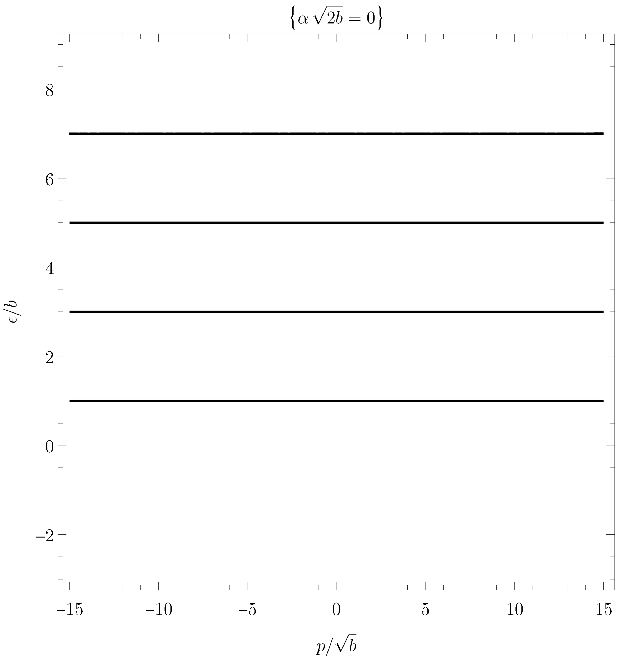
\includegraphics[width=0.45\textwidth]{grafy/dirac0.pdf}%
    \hspace{0.1\textwidth}%
    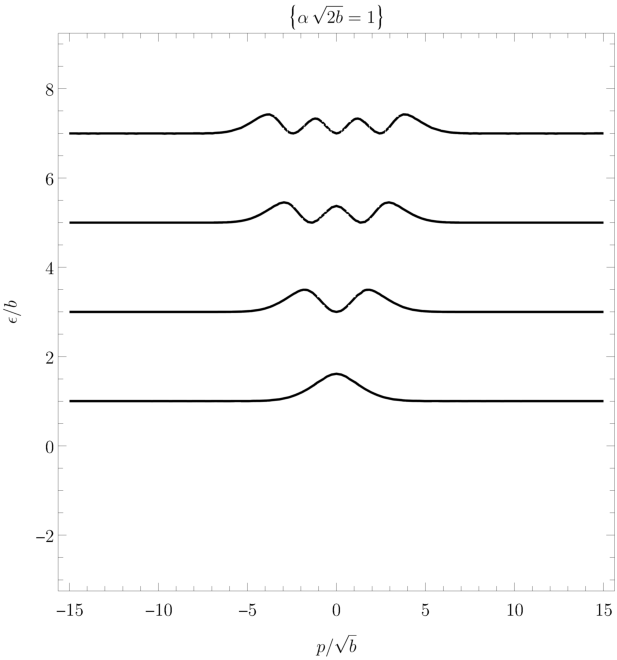
\includegraphics[width=0.45\textwidth]{grafy/dirac1.pdf}%
    \\[1em]%
    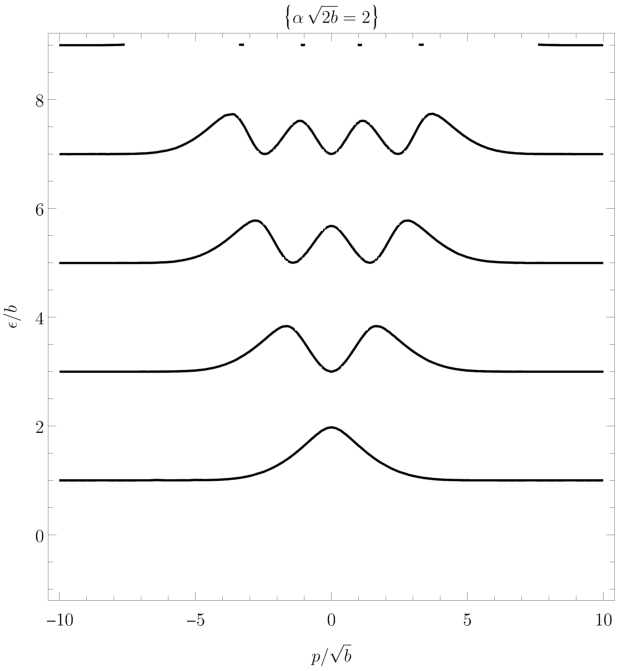
\includegraphics[width=0.45\textwidth]{grafy/dirac2.pdf}%
    \hspace{0.1\textwidth}%
    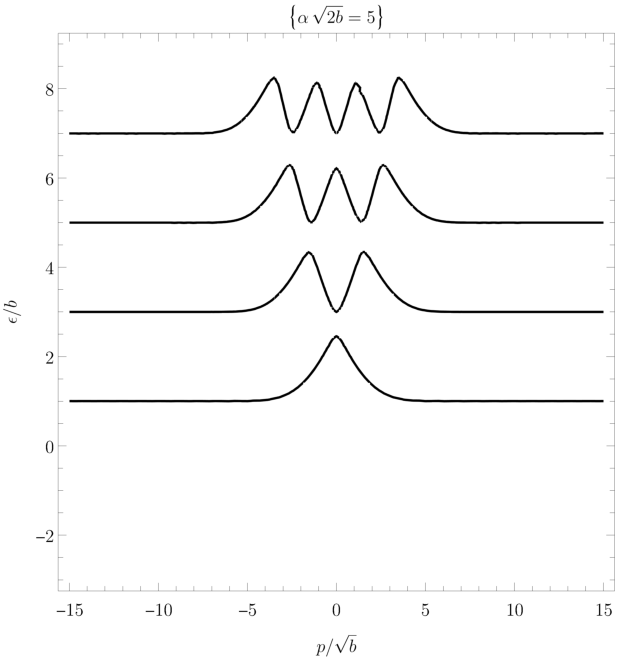
\includegraphics[width=0.45\textwidth]{grafy/dirac5.pdf}%
    \\[1em]%
    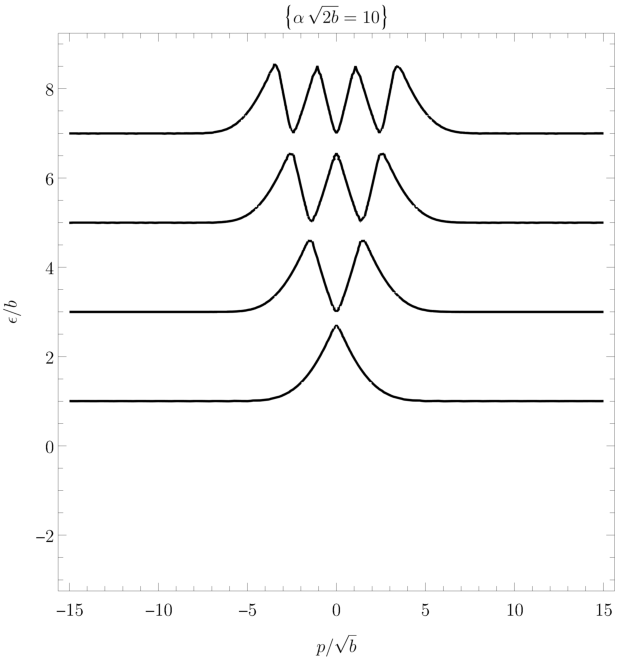
\includegraphics[width=0.45\textwidth]{grafy/dirac10.pdf}%
    \hspace{0.1\textwidth}%
    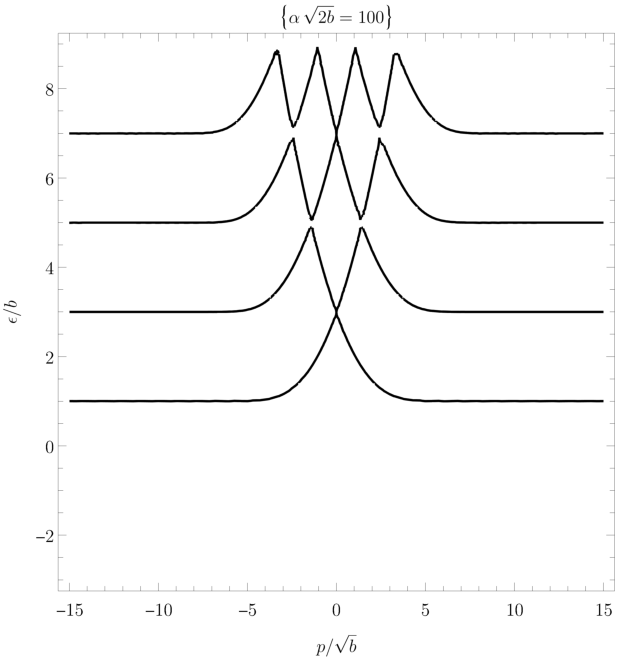
\includegraphics[width=0.45\textwidth]{grafy/dirac100.pdf}\par
    \caption{The first four energy levels $\epsilon$ as a function of the $y$-momentum $p$ for $\alpha\,\sqrt{2b} = 0, 1, 2, 5, 10$ and $100$ (starting with an unperturbed system, followed by an increasingly repulsive perturbation).}
    \label{plots-dirac-repulsive}
\end{figure}

\begin{figure}[p]
    \centering
    \noindent
    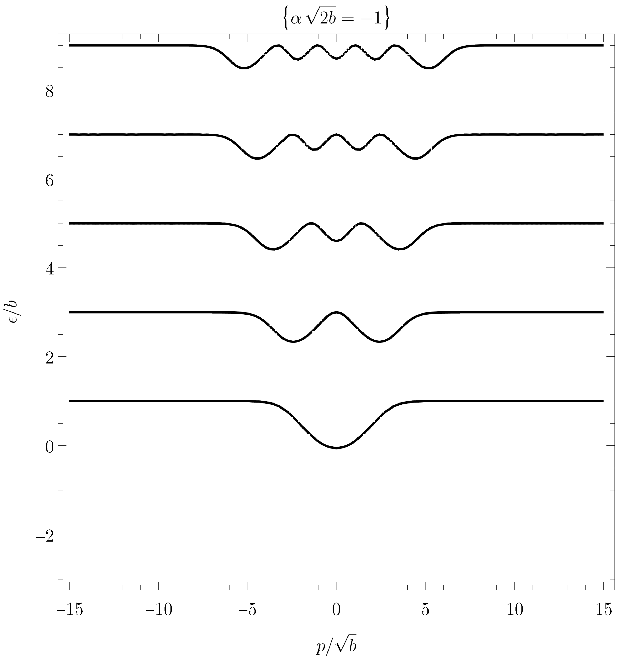
\includegraphics[width=0.45\textwidth]{grafy/dirac-1.pdf}%
    \hspace{0.1\textwidth}%
    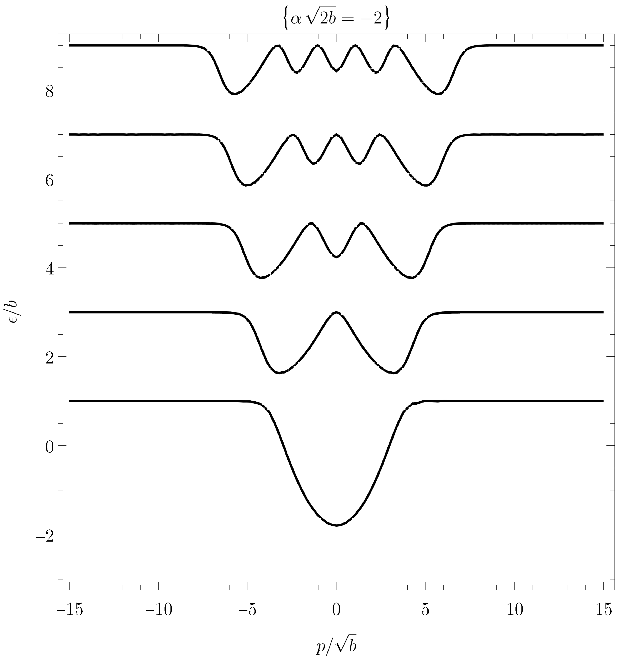
\includegraphics[width=0.45\textwidth]{grafy/dirac-2.pdf}%
    \\[2em]%
    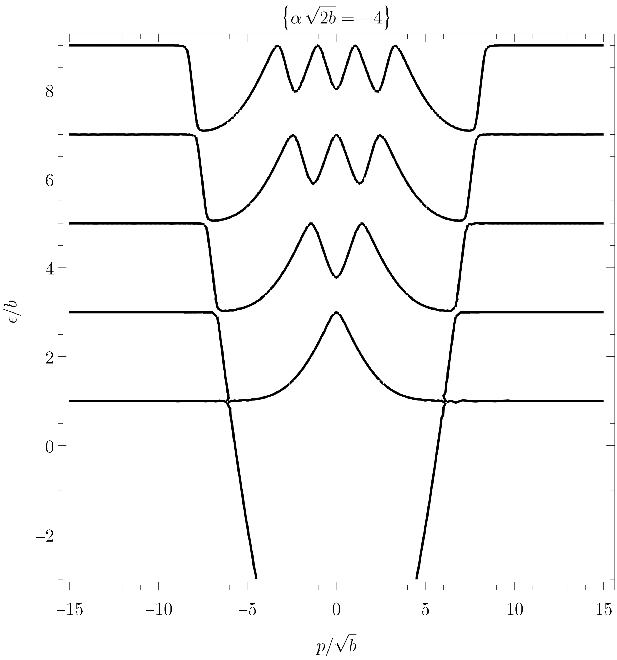
\includegraphics[width=0.45\textwidth]{grafy/dirac-4.pdf}%
    \hspace{0.1\textwidth}%
    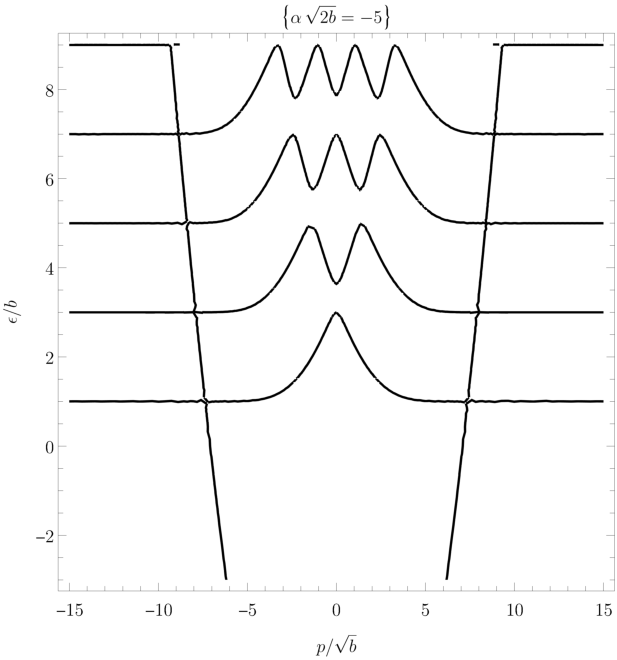
\includegraphics[width=0.45\textwidth]{grafy/dirac-5.pdf}\par
    \caption{The first five energy levels $\epsilon$ as a function of the $y$-momentum $p$ for $\alpha\,\sqrt{2b} = -1, -2, -4$ and $-5$ (system with an increasingly attractive perturbation).}
    \label{plots-dirac-attractive}
\end{figure}

